\chapter{Grundlagen}

% Grundlagen:


% - TrackSort Schüttgutsortierung
% - Kalman Filter
% - NN
% 	- RNN
% 	- LSTM

In diesem Kapitel soll eine kurze Einführung in die für das Verständnis der restlichen Arbeit benötigten Themengebiete gegeben werden.
Primär sollen zunächst allgemein neuronale Netze und einige ihrer speziellere Aspekte betrachtet werden 
bevor ein kurzer Blick auf das bei den Experimenten verwendete Schüttgutsortiersystem \textit{TableSort} geworfen wird. 

% hier Könnte man das Kalman Filter Kapitel einfügen
% \section{Das Kalman-Filter}
\todo[inline]{Entscheiden, ob diese Section komplett weg soll}
Als Kalman-Filter bezeichnet man ein mathematisches Verfahren mit dem Messfehler in realen Messwerten reduziert werden können und nicht messbare Systemgrößen geschätzt werden können. 


\todo{vergangene, aktuelle und zukünftige Systemzustände schätzen}
\todo{Einschränkung Linearität (Extended Kalman) und Gauß rauschen}

Der Zustand des Systems zum Zeitschritt \(t\) wird als \(y_t\) und die Messung im Zeitschritt \(t\) als \(z_t\) bezeichnet.

\begin{equation}
	y_t = A y_{t-1} + w, 	w \sim N(0, Q)
\end{equation}

\begin{equation}
	z_t = H y_{t} + v, 	v \sim N(0, R)
\end{equation}

Dabei ist \(A\) die Zustandsübergangsmatrix, die den Übergang von einem Zustand in den nächsten beschreibt.
\(H\) ist die Messmatrix, die beschreibt wie Messungen aus dem Zustand entstehen und Q und R sind die Kovarianzmatrizen des Systemrauschens beziehungsweise des Messrauschens. 

Das Kalman-Filter funktioniert mittels abwechselnd ausgeführter \textit{predict} und \textit{update} Schritte.

\begin{equation}
\hat{y}'_t = A \hat{y}'_{t-1}
\end{equation}

\begin{equation}
	\hat{P}'_t = A \hat{P}'_{t-1} A^\textit{T} + Q
\end{equation}






\section{Neuronale Netze}

Als Neuronale Netze  % beziehungsweise \textit{künstliche neuronale Netze}, wie sie manchmal korrekter genannt werden, 
bezeichnet man in der Informatik Systeme aus künstlichen Neuronen, die heute eine wichtige Rolle im Feld des maschinellem Lernen einnehmen.
Manchmal werden sie korrekter als \textit{künstliche neuronale Netze} bezeichnet um sie von \textit{natürlichen neuronalen Netzen} 
wie dem menschlichen Gehirn zu unterscheiden, nach deren biologischem Vorbild sie modelliert sind.

Die Grundsteine des Feldes wurde bereits 1943 von Warren McCulloch und Walter Pitts gelegt, 
die in ihrem Paper \cite{mcculloch1943logical} ein Neuronenmodell vorschlugen, mit dem sich logische arithmetische Funktionen berechnen lassen. 
Nach einer Periode von relativ geringer Aufmerksamkeit der wissenschaftlichen Gemeinschaft während den 1970ern und folgenden Jahrzehnten 
haben einige bahnbrechende Ergebnisse um das Jahr 2010, unter anderem im Feld der Spracherkennung, das Interesse an dem Feld wieder entfacht. 


% Nachdem jedoch Marvin Minsky und Seymour Papert zeigten, dass einzelne Perzeptrons nicht in der Lage sind linear nicht separierbare Probleme zu lösen sank das Interesse an dem Feld.

\subsection{{Perzeptron}}
Die kleinste Einheit eines neuronalen Netzes ist das Perzeptron, wie es 1958 von Frank Rosenblatt beschrieben wurde \cite{rosenblatt1958perceptron}.
Es ist eine Art künstliches Neuron, dass eine Reihe an Eingaben entgegen nimmt und einen einzelnen Wert \(o\) ausgibt.

\begin{figure}
    \centering
    % \missingfigure{Grafik Neuron}
	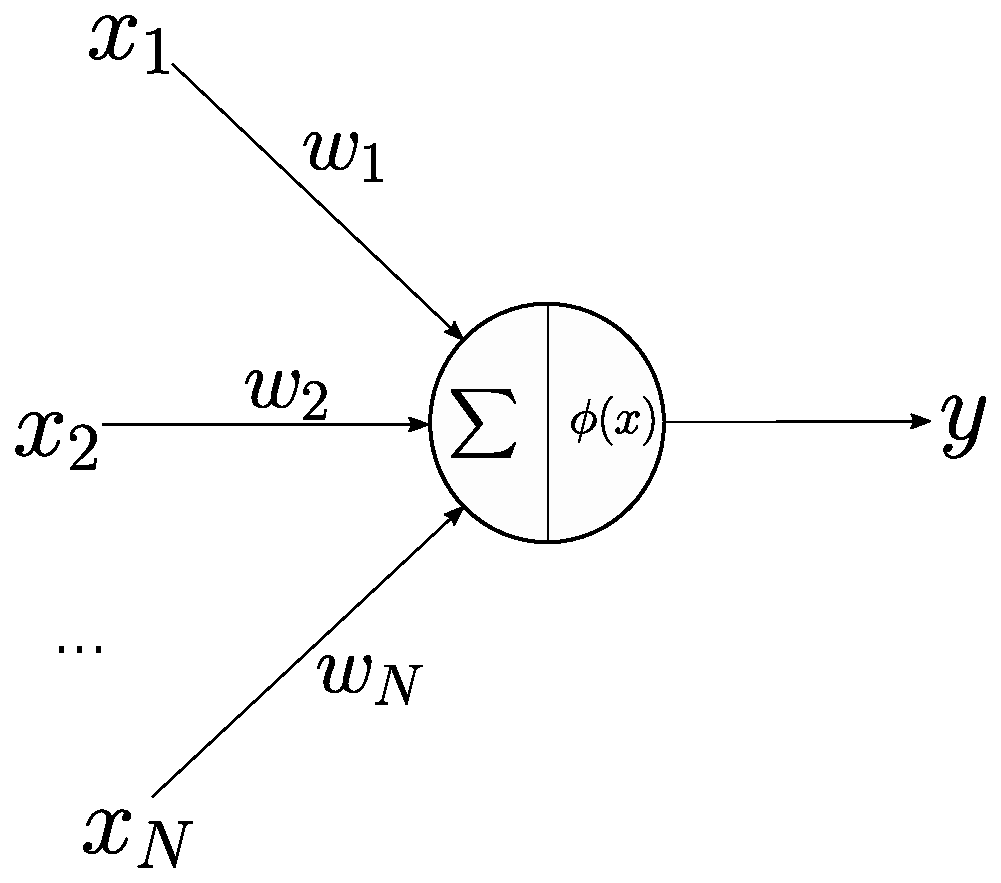
\includegraphics[width=0.5\textwidth]{perceptron-2}
	\caption{Schematischer Aufbau Neuron}
	% \todo{Quelle Bild!}
	\label{fig:singleNeuron}
\end{figure}

Die einzelnen Eingaben \(x_i\) haben jeweils eine Gewichtung \(w_i\).
Es existiert ein sogenannter Schwellwert oder \textit{bias}, der normalerweise 
durch eine zusätzliche Eingabe \(x_{m+1}\) mit dem Wert \(+1\) und dem dazugehörigen Gewicht \(w_{m+1}\) modelliert wird.
Den Ausgabewert \(y\) erhält man dadurch, dass man die gewichteten Eingaben aufsummiert und in die Aktivierungsfunktion \( \phi \) des Perzeptrons gibt.
Ein Überblick über verschiedene Aktivierungsfunktionen ist unter~\ref{sec:activationfuncs} zu finden.

Mathematisch ist die Ausgabe eines Perzeptrons also wie folgt definiert:

\begin{equation}
	y = \phi \Big( \sum_{i= 0}^{m} w_i x_i \Big)
\end{equation}

Beim Lernen werden die Gewichte der einzelnen Eingaben so an gepasst, dass die gewünschte Ausgabe erreicht wird.
Ein einzelnes Perzeptron mit zwei Eingängen kann zur Darstellung der logischen Operatoren AND, OR und NOT genutzt werden

Letztendlich ist ein solches Perzeptron jedoch nur ein linearer Klassifikator und kann somit zum Beispiel den XOR Operator nicht auflösen.
Dies zeigten Marvin Minksy und Seymour Papert 1969 in einflussreichen Buch \textit{Perceptrons: an introduction to computational geometry} \todo{quelle}
\todo{Linear Trennbares / Nicht-linear Trennbares Problem (AND vs XOR)}

Solche, nicht linear-separierbare Probleme zu lösen müssen mehrere Schichten an Neuronen kombiniert werden.

\subsection{Aktivierungsfunktionen}
\label{sec:activationfuncs}
\todo[inline]{Entscheiden, ob diese Section weg soll, oder auf nur ReLU reduziert werden sollte}
Es gibt verschiedene Aktivierungsfunktionen, die für den Einsatz in neuronalen Netzen in Frage kommen.
Sie sind von essenzieller Wichtigkeit, da ohne eine Nicht-Linearität das Netz in eine einfache Regression kollabiert.

Eine Aktivierungsfunktion sollte leicht abzuleiten sein, 
da dies im Rahmen des Trainings mit dem Backpropagation Algorithmus häufig geschieht und sonst beträchtlicher Rechenaufwand entsteht.

In der Vergangenheit wurden einige verschiedene Aktivierungsfunktionen verwendet.
% Einige häufig verwendete Aktivierungsfunktionen sollen hier vorgestellt werden.
Jede dieser Funktionen stellt eine Nicht-Linearität dar und nimmt eine einzelne Zahl, wendet eine bestimmte, festgelegte mathematische 
Operation auf diese an und gibt das Ergebnis zurück.
Historisch ist häufig die Sigmoid-Funktion verwendet worden, da sie das Verhalten eines natürlichen Neurons gut nachbildet.
\begin{equation}
	f(x) = \frac{1}{1 + e^x} = \frac{e^x}{e^{x + 1}}
	\label{func:Sigmoid}
\end{equation}
In der Praxis jedoch haben sich einige Nachteile der Sigmoid-Funktion gezeigt.
Einige dieser Probleme konnten mit der Verwendung des Tangens hyperbolicus  behoben werden, 
durchgesetzt haben sich jedoch in letzter Zeit sogenannte \textit{Rectified Linear Units}, oder kurz ReLUs.

% \begin{description}
	
	% hier Könnte man die Absätze zu Sigmoid und TanH einfügen
	% \item[Sigmoid-Funktion] \hfill \\
		\begin{equation}
			f(x) = \frac{1}{1 + e^x} = \frac{e^x}{e^{x + 1}}
			\label{func:Sigmoid}
		\end{equation}
		\begin{equation}
			f'(x) = f(x) * (1 - f(x))
		\end{equation}
		Die mathematische Form der Sigmoid Aktivierungsfunktion ist in Abbildung \ref{sigmoidFunc} zu sehen.
		Sie bildet die reellen Zahlen \(\mathbb{R}\) auf das Intervall \((0,1)\) ab. 
		Für betragsmäßig größer werdende negative Zahlen nähert sich der Rückgabewert \(0\) an,
		ebenso wie für größer werdende positive Zahlen sich der Rückgabewert an \(1\) annähert.

		Die Sigmoid Funktion ist eine historisch häufig genutze Funktion, da sie das Verhalten eines natürlichen Neurons,
		der biologischen Motivation für künstliche Neuronen, gut nachbildet:
		komplette Inaktivität eines Neurons bei Ausgabe 0 bis zum feuern mit maximaler Frequenz bei Ausgabe 1.

		In der Praxis jedoch haben sich einige Nachteile der Sigmoid Funktion gezeigt, weshalb sie quasi nicht mehr genutzt wird.
		Der gewichtigste von diesen ist, dass ihre Ableitung bei großen Beträgen beinah \(0\) ist.
		Dies führt dazu, dass während der Ausführung des Backpropagation-Algorithmus beinah keine Änderungen passieren und dementsprechend das Netz sehr langsam lernt.
		
		\begin{figure}
			\centering
			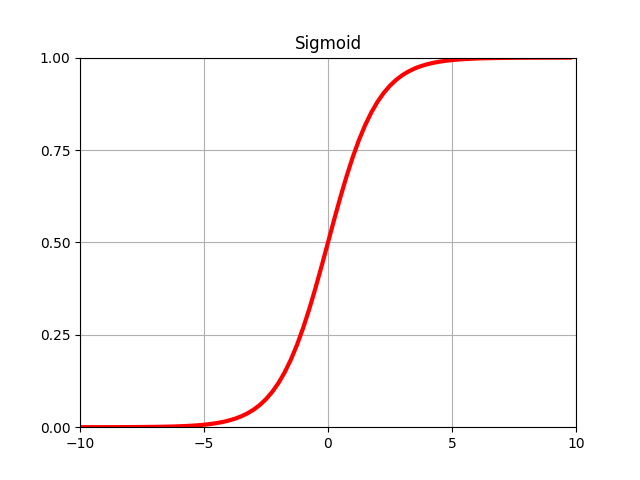
\includegraphics[width=0.618\textwidth]{Sigmoid}
			\caption{Plot der Sigmoid Funktion}
			\label{sigmoidFunc}
		\end{figure}
		  


	\item[TanH] \hfill \\
		\begin{equation}
			f(x) = \tanh(x) = \frac{e^x - e^{-x}}{e^x + e^{-x}}
		\end{equation}
		\begin{equation}
			f'(x) = 1 - f(x)^2
		\end{equation}
		Die TanH-Aktivierungsfunktion ist in Abbildung \ref{tanhfunction} dargestellt.
		Im Gegensatz zur Sigmoid Funktion bildet sie die reellen Zahlen \(\mathbb{R}\) auf das Intervall \((-1, 1)\) ab.
		Weil sie zentriert um den Nullpunkt ist, wird sie bei realen Anwendungen der Sigmoid Funktion vorgezogen.
		Das Saturationsproblem der Sigmoid Funktion besteht jedoch immer noch.
		\begin{figure}
			\centering
			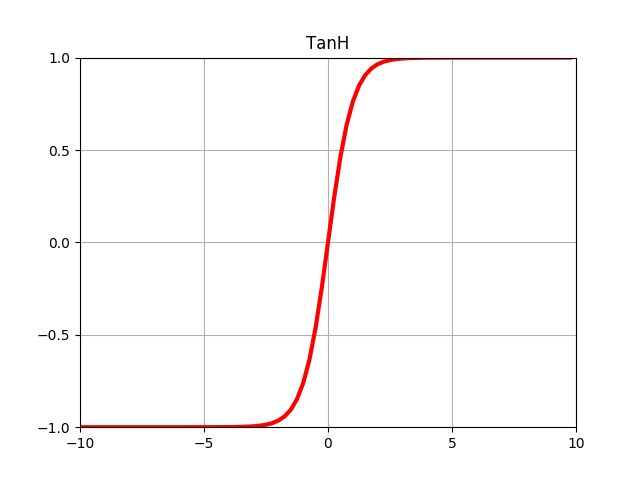
\includegraphics[width=0.618\textwidth]{Tanh}
			\caption{Plot der Tanh Funktion}
			\label{tanhfunction}
		\end{figure}
	
	% \item[ReLU] \hfill \\
\begin{equation}
	f(x) = \max(0, x)
\end{equation}
\begin{equation*}
	f'(x) = \begin{cases}
	0 &\text{, falls $x < 0$}\\
	1 &\text{, falls $x > 0$}
	\end{cases}
\end{equation*}
	Abbildung~\ref{reluoutput} zeigt den Plot einer solchen ReLU. 
	\todo{ReLU plot neu machen: dicker bei unter 0 und als Vector graphic statt als PNG}
	Die Aktivierung von ReLUs ist ein einfacher Schwellwert, der weit weniger rechenintensiv ist, als die aufwendigen Exponenzialfunktionen von Sigmoid und tanh.
	In der Praxis hat sich gezeigt zudem gezeigt, dass ReLus deutlich schneller konvergieren als Sigmoid- oder tanh-Neuronen.  
	Krizhevsky et al. haben in ihrem Paper~\cite{NIPS2012_4824} einen Geschwindigkeitsgewinn um Faktor 6 feststellen können.
	Ein Problem, das mit ReLUs jedoch existiert ist, dass einzelne Neuronen während dem Training "absterben" können.
	Diese Neuronen sind dann für jeden beliebigen Input inaktiv und können niemals wieder etwas zur Ausgabe des Netzes beitragen.
	Durch die Wahl einer geeigneten Lernrate oder den Einsatz sogenannter Leaky ReLUs lässt sich dies jedoch vermeiden.
	Leaky ReLUs haben im Gegensatz zu normalen ReLUs eine kleine positive Steigung im negativen Bereich.
	\begin{equation}
		f(x) = \begin{cases}
			x &\text{, falls } x  >  0\\
			0.01 x &\text{, falls } x  \leq  0
		\end{cases}
	\end{equation} 
	

	\begin{figure}
		\centering
		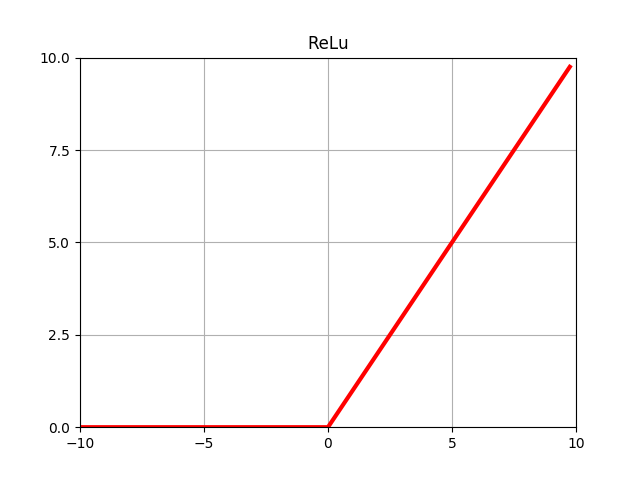
\includegraphics[width=0.618\textwidth]{ReLu}
		\caption{Plot der Ausgabe einer ReLU}
		\label{reluoutput}
	\end{figure}



% \end{description}

% \begin{figure}[h]
%     \centering
%     \begin{subfigure}[t]{0.3\textwidth}
% 		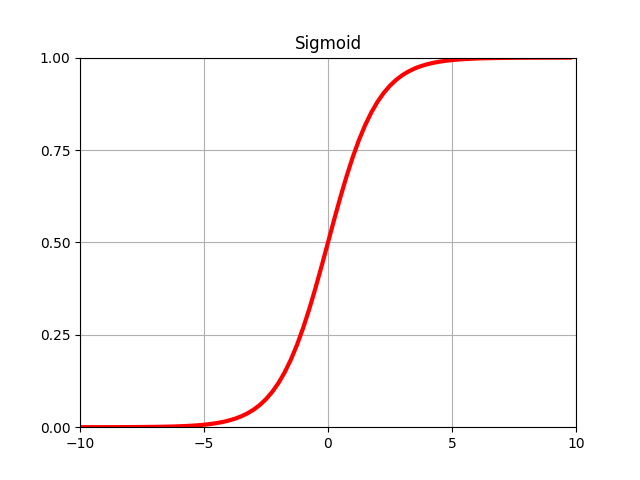
\includegraphics[width=\textwidth]{Sigmoid}
% 		\caption{Sigmoid Funktion}
%     \end{subfigure}
%     \begin{subfigure}[t]{0.3\textwidth}
% 		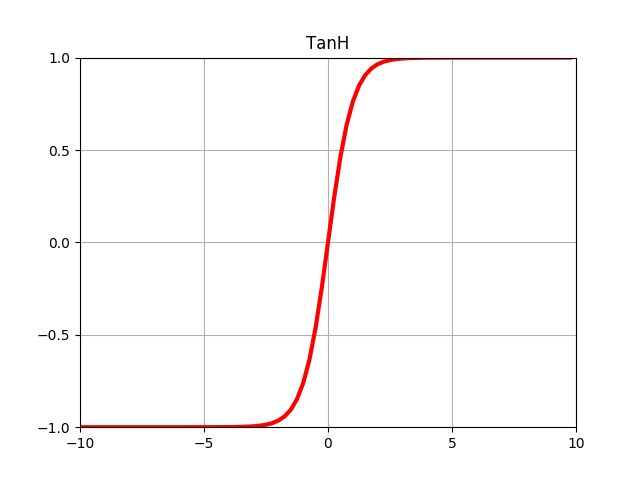
\includegraphics[width=\textwidth]{Tanh}
% 		\caption{TanH Funktion}
%     \end{subfigure}
%     \begin{subfigure}[t]{0.3\textwidth}
%         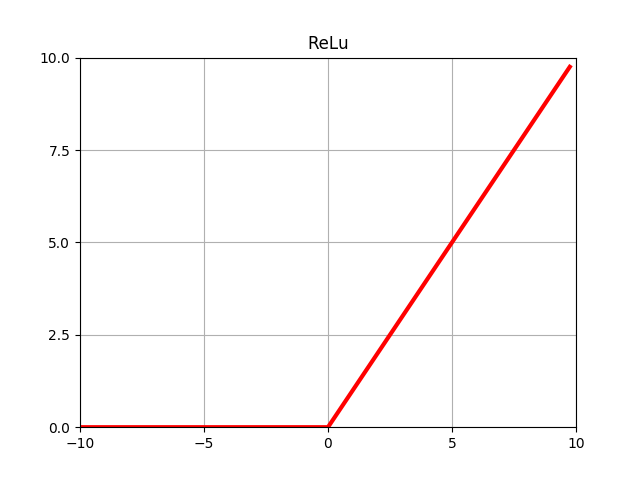
\includegraphics[width=\textwidth]{ReLu}
%         \caption{ReLU}
%     \end{subfigure}
%     \caption{Häufig verwendete Aktivierungsfunktionen}
%     \label{eval:function}
% \end{figure}



\subsection{Feedforward Netze}

% \textbf{absatz über Feedforward Netze. Basic}
\begin{itemize}
	\item Definition (keine Kreise oder Schleifen). (Kommentar Florian: \"Rückkopplung\")
	\item Gegenstück zum RNN
	\item grundlegende Architektur in Layern 
	\item Aktivierungsfunktionen in Layern
	\item Outputlayer: Verschiedene Aktivierungsfunktionen:
	\item Linear für regression, z.B. Softmax für Wahrscheinlichkeitsverteilung Softmax
\end{itemize}



Als Feedforward Netz bezeichnet man ein neuronales Netz, zwischen dessen Knoten keine Kreise oder Schleifen existieren.
Das entsprechende Gegenstück bezeichnet man als \textit{Rekurrentes Neuronales Netz}
Die Informationen wandert in der Verarbeitungsrichtung von den Eingabeknoten zu den Ausgabeknoten.
Für gewöhnlich sind die einzelnen Knoten in Schichten, sogenannten Layern, organisiert.
Die Neuronen eines einzelnen Layers sind meist 
Die Eingabe wird in ein Input Layer eingeben.

\subsection{Backpropagation}

\todo[inline]{Entscheiden ob die Subsection weg sollte}
Der Backpropagation Algorithmus ist ein Verfahren mit denen künstliche neuronale Netze in der Lage sind komplizierte Zielfunktionen einzulernen.
Es ist eine Methode, bei der effizient der Gradient der Fehlerfunktion in Abhängigkeit vom Gewicht der einzelnen Kanten im Netz bestimmt werden kann,
was dann für einen Gradientenabstieg verwendet werden kann. 

\begin{itemize}
	\item Definition und Beschreibung
	\item Nur supervised learning: Gradient der Fehlerfunktion wird benötigt \(\rightarrow\) Tatsächliches Ergebnis muss bekannt sein.
	\item "Finden einer Funktion, die am besten die Inputs auf die outputs mapt"
\end{itemize}

\subsection{Overfitting}

Das essenzielle Maß nachdenen neuronale Netze bewertet werden, ist wie gut sie mit neuen, unbekannten Daten umgehen, die nicht in den Trainingsdaten vorhanden waren. 
Diese Eigenschaft von Trainingsdaten auf unabhängige Testdaten zu schließen wird Generalisierung genannt. 

Als Overfitting bezeichnet man es, wenn ein Modell sich zu sehr an ein gegebenes Datenset anpasst und 
dafür in Kauf nimmt zusätzliche oder zukünftige Daten schlechter zu repräsentieren.
Das System wird also schlechter darin zu generalisieren.

Im Feld des überwachten Lernens beziehungsweise der neuronalen Netze ist Overfitting daran zu erkennen,
dass die Qualität die Ausgaben des Netzes auf dem Trainingsdatenset sich weiter verbessert,
während sie auf dem Testdatenset schlechter wird.
Dies kann zum Beispiel der Fall sein, wenn das Modell Rauschen in den Testdaten als Teil der zugrundeliegenden Struktur interpretiert. 


Dem Overfitting gegenüber steht das Underfitting. 
Als Underfitting bezeichnet man wenn das Netz nicht in der Lage ist
eine ausreichend gute Performance auf den Trainingsdaten zu erreichen.
Das kann passieren wenn das Modell nicht ausreichend komplex ist um die zugrundeliegende Struktur der Daten abzubilden.


Sowohl Overfitting als auch Underfitting hängen mit der Kapazität eines Netzes zusammen.
Ist die Kapazität zu gering kann es sein, dass das Netz daran scheitert die Trainingsdaten zu lernen.
Ist die Kapazität zu groß, so kann es passieren, dass das Netz, umgangsprachlich ausgedrückt, die Trainingsdaten einfach auswendig lernt.

Dies ist beispielhaft in Abbildung~\ref{fig:capacity} zu sehen.
Aus der zugrundeliegenden \( \cos \)-Funktion werden Stichproben mit einem Rauschterm entnommen. 
Stellvertretend für das Lernen mit neuronalen Netzen wird hier lineare Regression benutzt,
um die Parameter eines Polynoms zu lernen.
Die Kapazität des Modells wird hier durch den Grad des Polynoms festgelegt.

In Abbildung~\ref{subfig:underfitting} wird ein Polynom mit dem Grad 1 gelernt.
Die Kapazität ist zu niedrig und dementsprechend schafft das Modell es nicht einmal die Stichproben akkurat zu repräsentieren.

In Abbildung~\ref{subfig:rightfitting} ist der Grad des Polynoms 4.
Das resultierende Modell ist relativ dicht an der ursprünglichen Funktion.

In Abbildung~\ref{subfig:overfitting}

\begin{figure}[h]
    \centering
	
	\begin{subfigure}[t]{0.6\textwidth}
		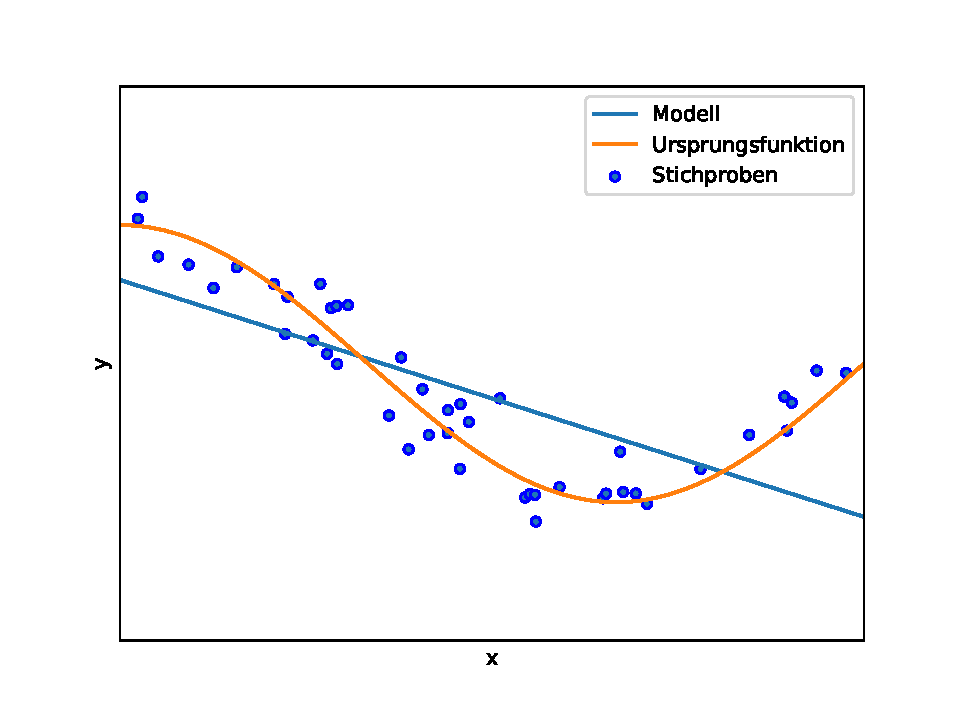
\includegraphics[width=\textwidth]{plotUnderfitting.pdf}
		\caption{Underfitting}
		\label{subfig:underfitting}
	\end{subfigure}
	% \quad
	\begin{subfigure}[t]{0.6\textwidth}
		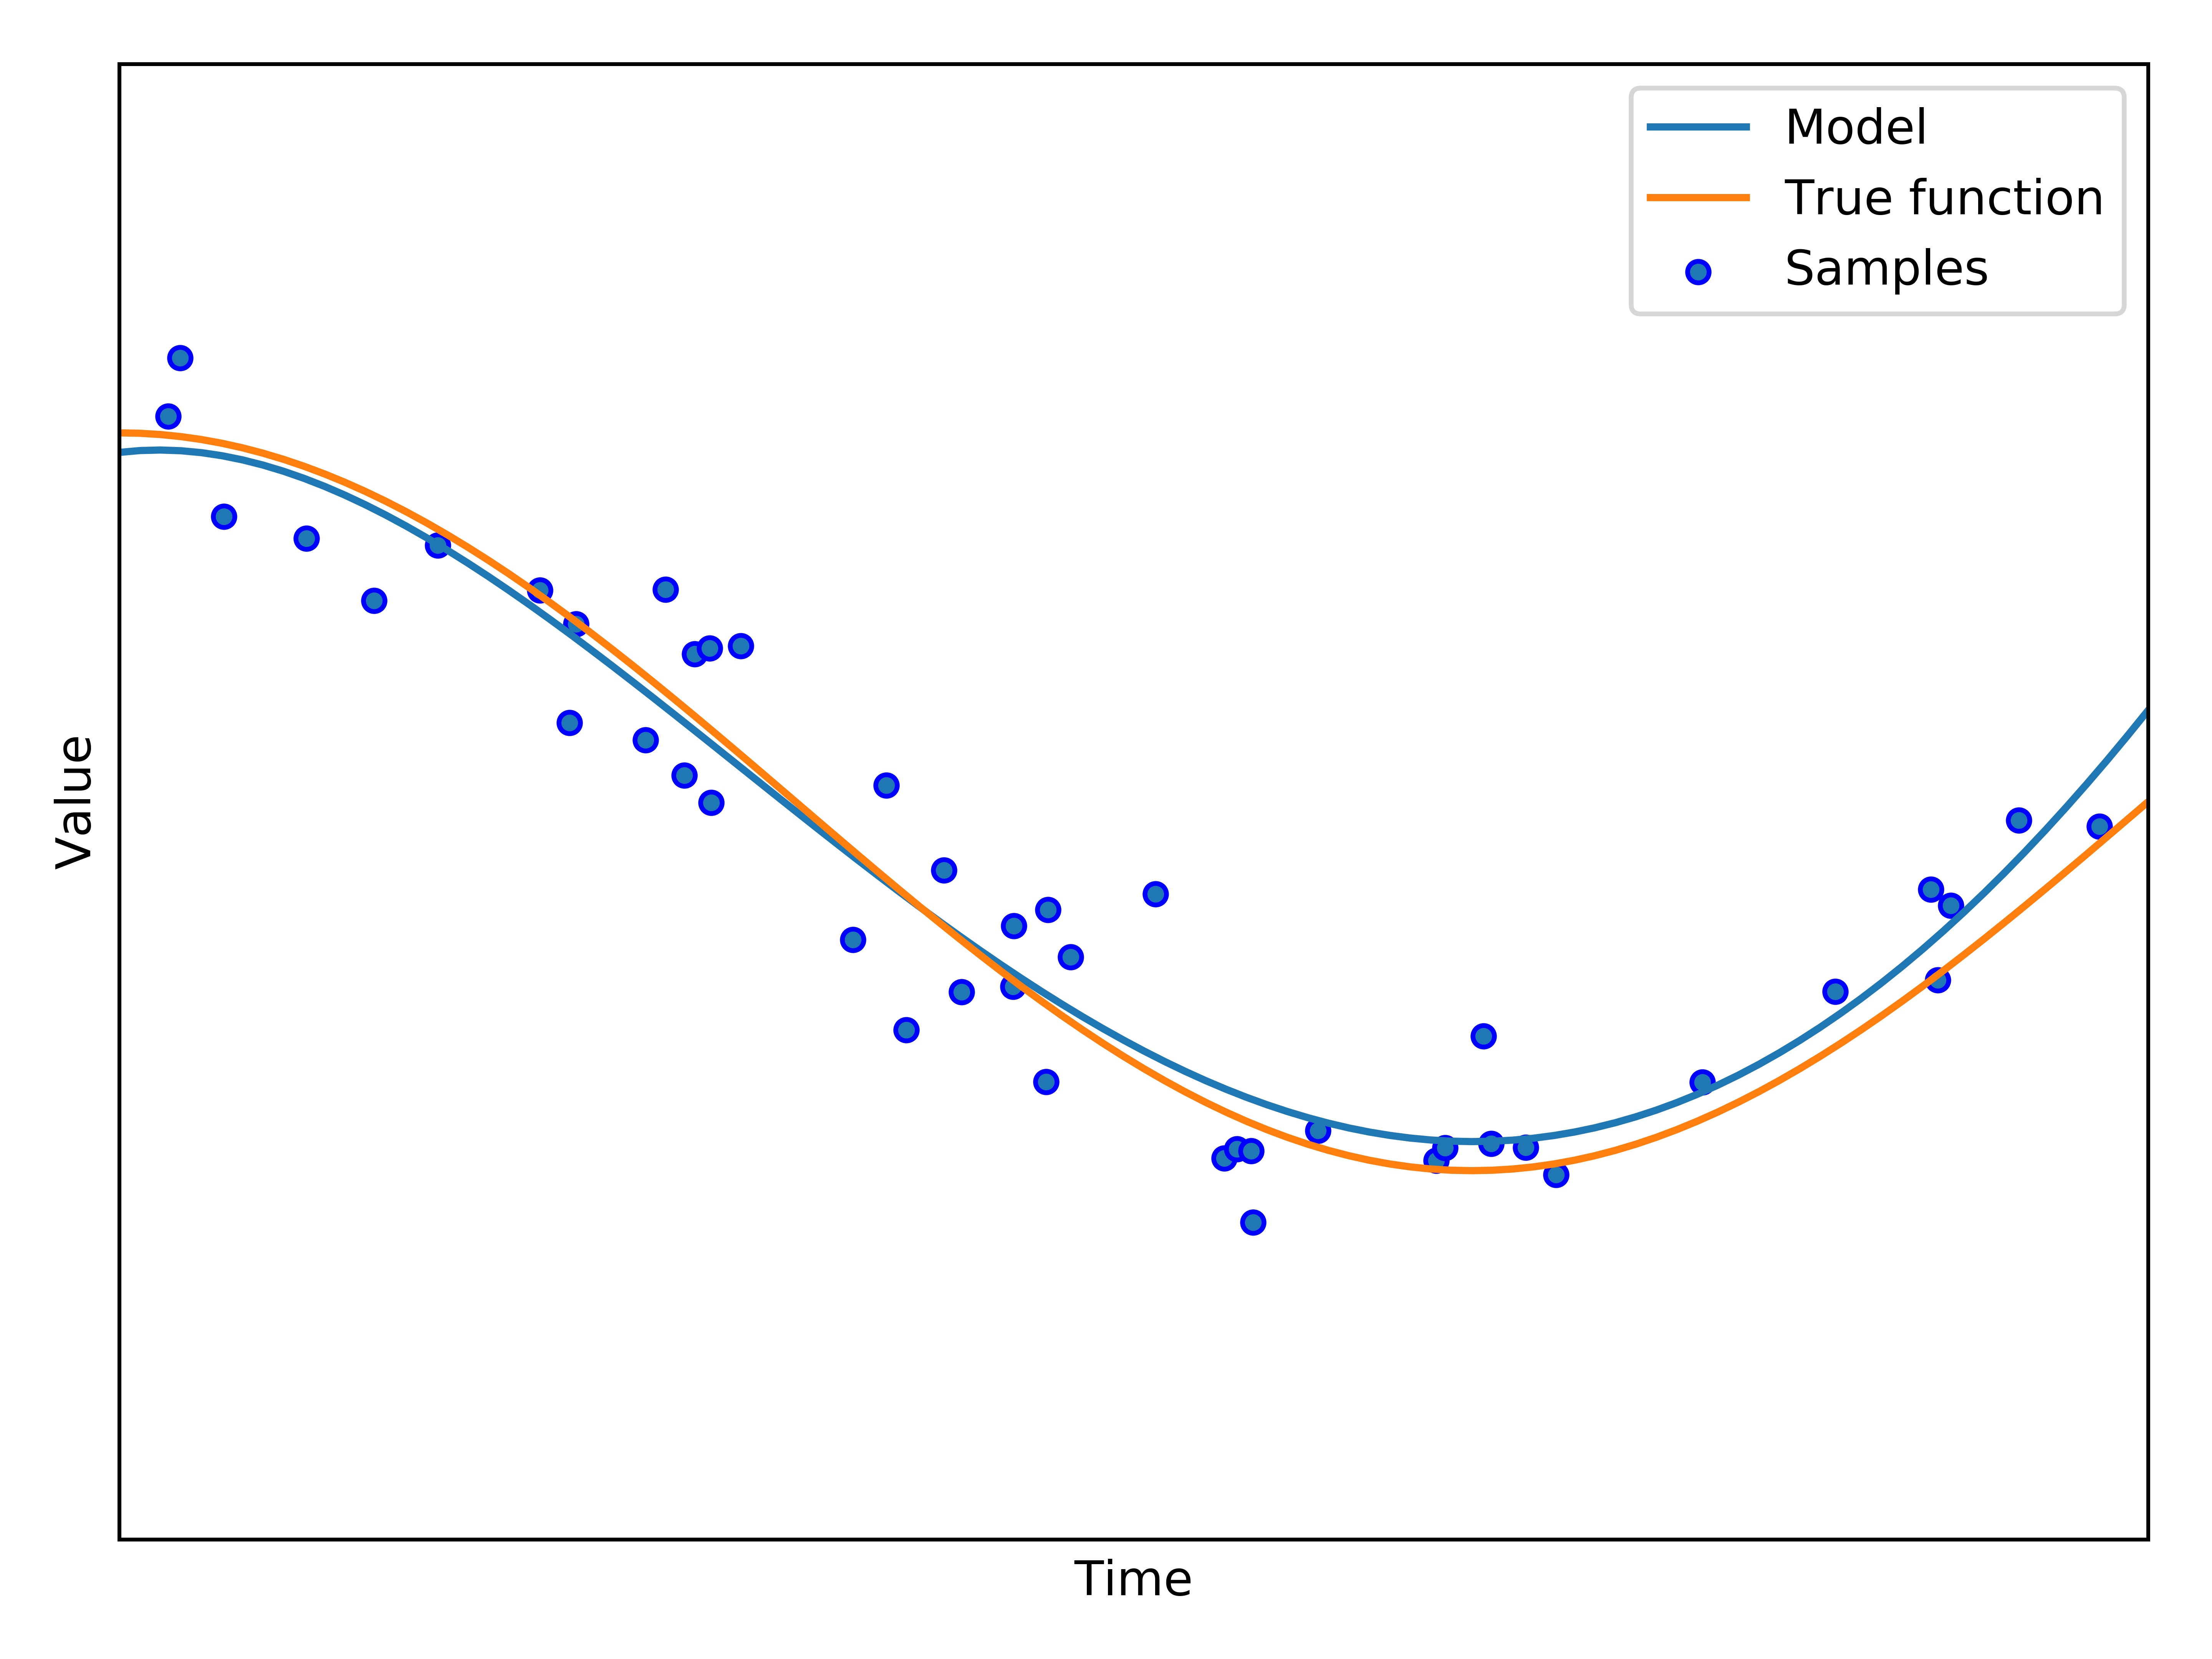
\includegraphics[width=\textwidth]{plotPassendesModell.pdf}
		\caption{Passendes Modell}
		\label{subfig:rightfitting}
	\end{subfigure}
	% \quad
	\begin{subfigure}[t]{0.6\textwidth}
        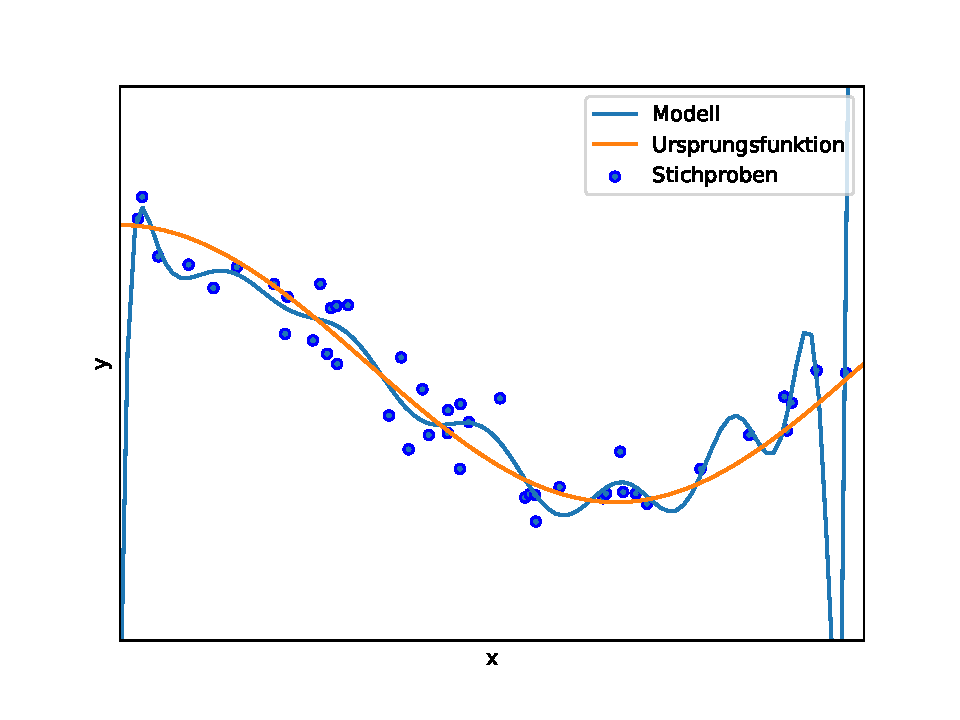
\includegraphics[width=\textwidth]{plotOverfitting.pdf}
		\caption{Overfitting}
		\label{subfig:overfitting}
	\end{subfigure}
	\caption{Visualisierung von unterschiedliche Kapazitäten}
	\label{fig:capacity}
\end{figure}

\begin{itemize}
	\item Methoden um Overfitting zu vermeiden:
	\item Mehr Trainingsdaten (z.B. durch Data-Augmentation)
	\item Regularisierung (L1, \(L_2\) (siehe unten), dropout)
\end{itemize}


\subsection{Regularisierung}

\begin{itemize}
	\item Regularisierung Definition
	\item Mathematische Formel Darstellung
	\item \(L_1\) und \(L_2\) Regularisierung
	\item L0 - warum nicht?
	\item (Maybe Dropout)
	\item Early Stopping? (das internet sagt, es ist eine art von Regularisierung und falls ich sie verwenden sollte, sollte ich sie hier erwähnen)
\end{itemize}

Als Regularisierung bezeichnet man eine Technik, die benutzt wird um ein Modell von Overfitting abzuhalten.
Sie wird in der Hoffnung angewendet, dass das Modell mit Regularisierung besser generalisiert als ohne.

Eine Möglichkeit ist, dass zur Loss Funktion ein Regularisierungsterm \(R\) hinzugefügt wird, 
der die Kosten basierend auf der Komplexität des Systems erhöht.

\begin{equation}
	\min_f \sum\limits_{i=1}^{m} V(f(\vec{x}_i), \vec{y}_i) + \lambda R(f)
\end{equation} 

Dabei ist \(V\) die Loss Funktion, beispielsweise \textit{Mean-Square-Error} oder \textit{Mean-Absolute-Error}.
\(n\) ist die Anzahl der Feature-Label-Paare,
\(x_i\) und \(y_i\) sind die einzelnen Eingabefeatures und das dazugehörige Label.
Die Funktion \(f\) ist in unserem Fall das neuronale Netz, das die Features entgegen nimmt.
\(\lambda\) ist ein Parameter, der die Gewichtung des Regularisierungsterm festlegt.
Wählt man diesen Parameter zu klein, so kann es sein, dass das Modell trotz Regularisierung noch immer overfittet.
Wählt man ihn zu groß so kann es sein, dass das Modell das Problem nicht mehr korrekt abbildet und es zu Underfitting kommt.
Der Regularisierungsterm \(R\) wird so gewählt, dass er die Komplexität der Funktion \(f\) wiederspiegelt.
Ein gutes Maß für die Komplexität eines neuronalen Netzes sind die Gewichte zwischen den Neuronen.
Beispiele für \(R\) wären zum Beispiel die \(L_1\)- oder die \(L_2\)-Regularisierung. % die jeweils mit der \(L_1\) beziehungsweise mit der \(L_2\)-Norm arbeiten.
Der entscheidende Unterschied zwischen den beiden ist der unterschiedliche Strafterm, zu sehen in~\ref{eqn:MSE-L1} für \(L_1\) und~\ref{eqn:MSE-L2} für \(L_2\). 
Die Fehlerfunktionen sind jeweils MSE mit dazugehörigen Strafterm.

\begin{equation} \label{eqn:MSE-L1}
	J(X, Y) = \frac{1}{m} \sum_{i=1}^{m} (\vec{y}^{(i)} - \hat{\vec{y}}^{(i)})^2 + \sum_{j, k} (|\mat{W}_{j,k}|)
\end{equation} 

\begin{equation} \label{eqn:MSE-L2}
	J(X, Y) = \frac{1}{m} \sum_{i=1}^{m} (\vec{y}^{(i)} - \hat{\vec{y}}^{(i)})^2 + \sum_{j, k} (\mat{W}_{j,k}^2)
\end{equation} 


Ein Regressionsmodell, dass \(L_1\)-Regularisierung verwendet wird auch als Lasso-Regression bezeichnet, 
während ein Modell mit \(L_2\)-Regularisierung als Ridge Regression beschrieben werden kann.
Vergleicht man die beiden Ansätze, so schrumpft die \(L_1\) Norm weniger wichtige Gewichte auf 0, was zu dünn besetzten Gewichtsvektoren führt.
Dies kann eine wünschenswerte Eigenschaft sein.
Im Gegensatz dazu hat die \(L_2\)-Regularisierung, den Vorteil, dass sie effizienter berechnen kann.
Der Strafterm von \(L_2\) hat eine geschlossene Form und kann in Form einer Matrix angewendet werden, während die Funktion von \(L_1\) auf Grund des Betrags eine nicht-differenzierbar ist.


\todo{absatz zu (L0 und warum man es nicht benutzt?)}

Eine weitere Regularisierungstechnik ist Dropout~\cite{JMLR:v15:srivastava14a}.
Dabei werden während dem Training eines neuronalen Netzes 
mit einer festgelegten Wahrscheinlichkeit zufällig Neuronen und die dazugehörigen Verbindungen abgeschaltet, 
wie in Abbildung~\ref{fig:dropout} dargestellt.
Dies soll insofern Overfitting vermeiden, dass es übermässige Kodaption von mehreren Neuronen erschwert.
Dropout als Technik wird insbesondere bei tiefen neuronalen Netzen eingesetzt. 

\begin{figure}[h]
    \centering
    \begin{subfigure}[t]{0.4\textwidth}
		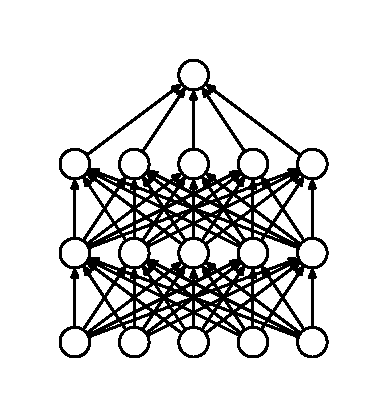
\includegraphics[width=\textwidth]{neuralNet}
		\caption{Unverändertes neuronales Netz}
    \end{subfigure}
    \begin{subfigure}[t]{0.4\textwidth}
		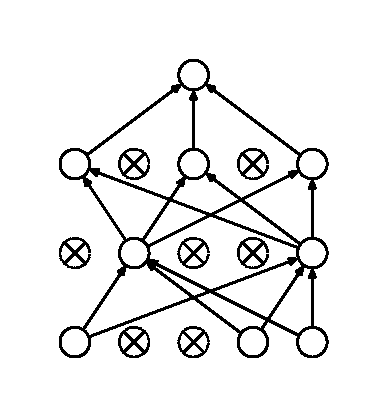
\includegraphics[width=\textwidth]{neuralNet_dropped}
		\caption{Nach Dropout Anwendungen.}
	\end{subfigure}
    \caption{Beispiel Dropout-Regularisierung~\cite{JMLR:v15:srivastava14a}}
    \label{fig:dropout}
\end{figure}


\section{TableSort System}

\todo[inline]{Viel stuff über das TableSort System}

\begin{itemize}
	\item kleiner, experimenteller Bandsortierer~\cite{doll2015}
	\item Entstanden in Kooperation zwischen dem Fraunhofer IOSB, Abteilung Sichtprüfsysteme, und dem Institut für Intelligente Sensor Aktor Systeme des Karlsruher Institut für Technologie.
	\item Im Rahmen des \textit{TrackSort} Projekts
	\item Gedacht für Experimente, wenn es zu aufwendig ist das mit dem großen großen zu machen und zum Mitnehmen auf Messen.
	\item 2 Modi: mit Förderband und mit Rutsche
	\item Mit Flächenkamera für TrackSort als auch die Zeilenkamera sind dargestellt.
	\item Ringlicht (Refence später)
	\item Die Zeilenkamera wird zurzeit in industriellen Schüttgutsortieranlagen verwendet, ist aber nicht optimal (Siehe all die Literatur)
\end{itemize}

Das Table

\begin{figure}
	% \missingfigure{Bild von TablesortSystem}
	\includegraphics[width=\textwidth]{TrackSortPic}
	\caption{TableSort Schüttgutsortiersystem [TODO Quelle]}
	% \todo{Quelle Bild!}
	\label{fig:tablesortsystem}
\end{figure}


\begin{figure}
    \centering
    \def\svgwidth{\columnwidth}
	\input{img/Aufbau-moved.pdf_tex}
	\label{fig:aufbau_tablesort}
	\caption{Schematische Darstellung des optischen Bandsortierers TableSort nach~\cite{Pfaff2017}.}
\end{figure}


